\documentclass[a4paper, parskip, twoside]{scrartcl}

\usepackage[swedish]{babel}
\usepackage[T1]{fontenc}
\usepackage[utf8]{inputenc}

\usepackage[light]{kpfonts}

\usepackage{amsmath}
\usepackage{amsfonts}
\usepackage{amssymb}

\usepackage{graphicx}

%%%%%%%
% TIKZ %
%%%%%%%%%

\usepackage{tikz}
\usetikzlibrary{shapes,arrows}

\usepackage{pgfplots}

\tikzstyle{decision} = [diamond, draw, fill=blue!20, 
    text width=5.5em, text badly centered, node distance=3cm, inner sep=0pt]
\tikzstyle{block} = [rectangle, draw, fill=blue!20, 
    text width=6em, text centered, rounded corners, minimum height=4em]

%%%%%%%%%
% TIKZ %
%%%%%%%

\usepackage{booktabs}

\newcommand{\dd}[2]{\frac{d #1}{d #2}}

\usepackage{float}
\usepackage{capt-of}

\usepackage{listings}
\usepackage{color}

\definecolor{matcom}{rgb}{0.0,0.5,0.0} 
\definecolor{matkey}{rgb}{0.0,0.0,1.0} 
\definecolor{matstr}{rgb}{0.0,0.5,0.0} 
\definecolor{matbg}{rgb}{0.9,0.9,0.9}

\lstset{language=Matlab,
basicstyle=\ttfamily,
inputencoding=utf8,
showstringspaces=false,
numberstyle=\ttfamily,
keywordstyle=\color{matkey},
stringstyle=\color{matstr},
commentstyle=\color{matcom},
backgroundcolor=\color{matbg},
frame=lines,
breaklines=true,
literate=%
{å}{{\r{a}}}1
{ä}{{\"a}}1
{ö}{{\"o}}1
{Å}{{\r{A}}}1
{Ä}{{\"A}}1
{Ö}{{\"O}}1
}

\usepackage{fancyhdr}
\pagestyle{fancy}

\fancyhead{}
\fancyfoot{}

\fancyhead[LE, RO]{P. Engström och N. Proos Vedin}
\fancyhead[LO, RE]{\slshape \leftmark\/}
\fancyfoot[LE, RO]{\thepage}

\usepackage[expansion=false, tracking=false, protrusion=true]{microtype}

\addtokomafont{disposition}{\rmfamily}

\title{\sc Miniprojekt 2 \\ \emph{Genetisk oscillator}}
\date{\today}
\author{Nathalie Proos Vedin \& Per Engström}

\usepackage{lipsum}
\begin{document}
%\maketitle
%\thispagestyle{empty}
\begin{center}

\vspace*{5cm}

\resizebox{0.7\textwidth}{!}{\Huge \bf Miniprojekt 2}

\emph{\Large Beräkninsvetenskap II}

\rule{0.7\textwidth}{1pt}

Per \textsc{Engström} \& Nathalie \textsc{Proos Vedin}

\today

\end{center}

\thispagestyle{empty}


\newpage
\tableofcontents
\thispagestyle{empty}

\newpage
% !TeX spellcheck = sv_SE
\section{Inledning}
\label{sec:inledning}
För att anpassa sig till dygnets cykliska beteende använder sig många organismer av en så kallad cirkadisk rytm, vilket är en biologisk klocka med en period på 24 timmar. I en förenklad modell över hur denna klocka fungerar kan rytmen sägas bero på två specifika, reglerande proteiner, ett som undertrycker (repressor, i rapporten nämnd protein R) och ett som aktiverar (activator, protein A) relevanta processer. Undersökningar visar att oscillatorns beteende till största del beror på två faktorer: koncentrationen av protein R och molekylärdynamiken i processen då protein A bildar ett inaktivt komplex med R \cite{ref:rapport}.

Syftet med detta miniprojekt var att utnyttja \emph{Gillespies algoritm} på det studerade systemet för att avgöra hur den stokastiska metodens resultat skiljer sig från den tidigare använda \cite{ref:bestarapportenyao} deterministiska metoden. Resultaten för två olika värden på nedbrytningshastigheten för protein R skulle jämföras och allmänna skillnader mellan de både metoderna skulle studeras.

\lipsum[1]
\section{Matematisk modell}
\label{sec:modell}

Den cirkadiska rytmen utgörs av 18 reaktioner som beskrivs i ekvation~20 (sidan 21) i \cite{hellander}. Varje reaktion $r$ har en tillhörande propensitet $w_r$ som beskriver hur frekvent reaktionen är. Varje reaktion kan beskrivas algebraiskt som en differens $n_r$ som beskriver hur varje partikel förbrukas eller produceras.

Propensiteterna $w_r$ är funktioner av tillståndet $x$. Givet $w_r$ för varje reaktion kan vi tala om den \emph{totala propensiteten} $\beta$ som är summan av varje enskild reaktions propensitet. Då kommer väntetiden mellan två reaktioner $\tau$ vara exponentialfördelad med parameter $\beta$.

Om vi jämför med \textsc{miniprojekt 1} så har vi övergått från koncentration av ämnen och deras  till en diskret modell där varje reaktion har en viss sannolikhet att inträffa. Sannolikheten att reaktionen $r$ sker i intervallet $[t, t + \tau]$ är $w_r \beta^{-1}$.
\lipsum[2]
% !TeX spellcheck = sv_SE
\section{Numeriska metoder}
\label{sec:metoder}

\begin{figure}
	\centering
	\resizebox{\textwidth}{!}{
		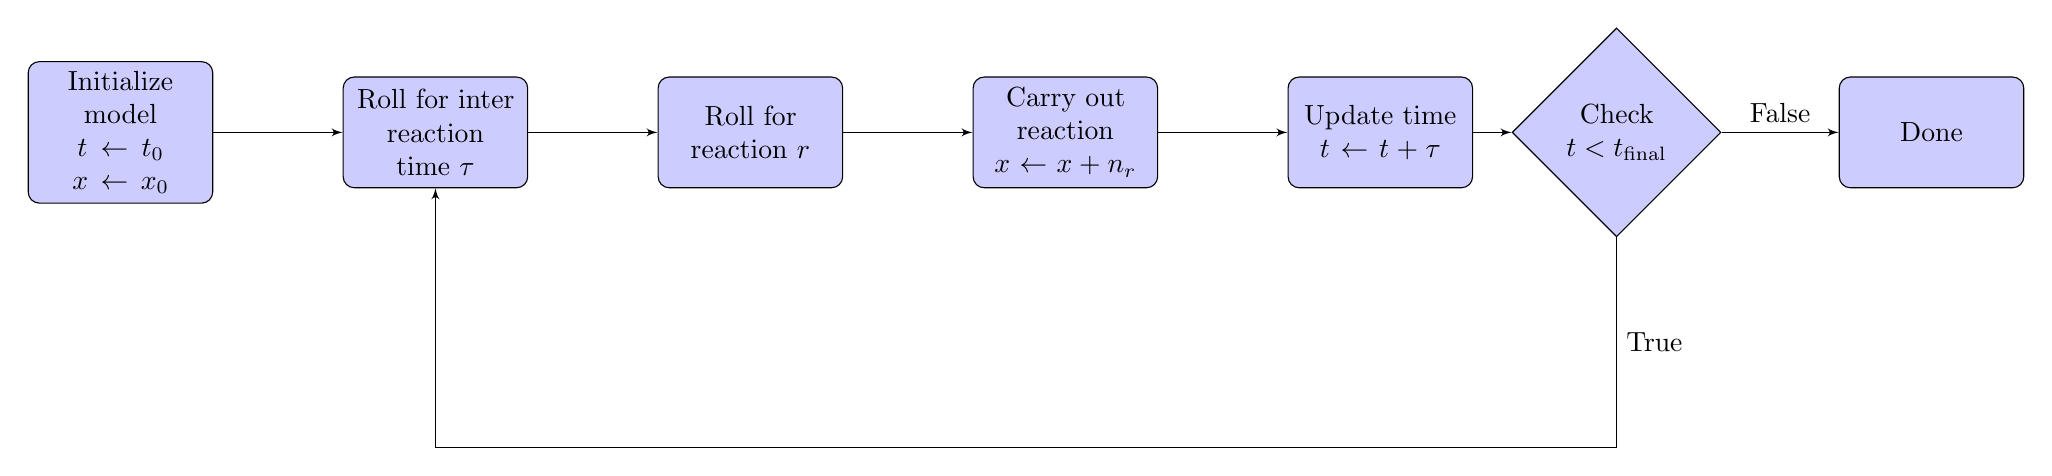
\begin{tikzpicture}[node distance=4cm, auto]
		\node [block](init) {Initialize model \\*
			$t \leftarrow t_0$ \\*
			$x \leftarrow x_0$};
		\node [block, right of=init] (timestep) {Roll for inter reaction time $\tau$};
		\node [block, right of=timestep] (reaction) {Roll for reaction $r$};
		\node [block, right of=reaction] (execute) {Carry out reaction \\*
			$x \leftarrow x + n_r$ };
		\node [block, right of=execute] (increase) {Update time \\*
			$t \leftarrow t + \tau$};
		\node [decision, right of=increase] (condition) {Check \\*
			$t < t_\mathrm{final}$};
		\node [block, right of=condition] (done) {Done};
		\coordinate [below of=condition] (null);
		
		
		\draw [-latex'] (init) -- (timestep);
		\draw [-latex'] (timestep) -- (reaction);
		\draw [-latex'] (reaction) -- (execute);
		\draw [-latex'] (execute) -- (increase);
		\draw [-latex'] (increase) -- (condition);
		\draw [-latex'] (condition) -- node [above] {False} (done);
		\draw [-latex'] (condition) -- node [right] {True} (null) -| (timestep);
		
		\end{tikzpicture}
	}
	\caption{Schematisk beskrivning av \emph{Gillespies algoritm}. I varje steg slumpas ett tidssteg $\tau \sim \exp(\beta)$ och en reaktion $r$ viktat efter deras propensiteter. Slutligen uppdateras tiden $t$ och tillståndet $x$.}
	\label{fig:gill}
\end{figure}

Till skillnad från \textsc{miniprojekt 1} där vi med ordinära
differentialekvationer arbetade deterministiskt, använde vi nu en
stokastisk metod. Detta krävde dock en omskrivning av den matematiska
modellen (se avsnitt 2).

Den ursprungliga kontinuerliga och deterministiska metoden baserades på
lösning av differentialekvationer som beskrev koncentrationen av de intressanta
partiklarna. Detta antar att antalet partiklar är stort så att koncentrationen
är approximativt kontinuerlig. I en cell är dock det antagandet svårt att
motivera, ty antalet av varje partikel kan finnas i endast ett fåtal exemplar.

Vi använde instället den diskreta och stokastiska \emph{Gillespies algoritm}. En beskrivning av algoritmen ses i figur~\ref{fig:gill}. Nu arbetar vi
direkt med partiklars antal istället för koncentrationer, och istället för
reaktionshastigheter har vi sannolikheter (propensiteter) för varje reaktion.

\subsection{Hitta tiden till nästa reaktion}

Först initierar vi vårt tillstånd med initialvärden för tiden $t$ (\lstinline|t|) och tillståndet $x$ (\lstinline|x|) enligt avsnitt~4. Sedan beräknar vi propensiteterna $w_r$ enligt \lstinline|w = prop_vilar(x, b)| där \lstinline|b| är en parametervektor enligt avsnitt~4 och \lstinline|w| är en $18 \times 1$-kolumnvektor. Vi kan då beräkna summan $\beta$ som \lstinline|beta = sum(w)|.

Sedan slumpar vi fram $\tau$ med hjälp av att invertera den kumulativa sannolikhetsfördelningen. Detta görs med ett slumptal $u_1 \sim U[0,1]$ enligt
\begin{equation}
\tau = \frac{-\ln u_1}{\beta} \, .
\end{equation}
Detta implementerar vi i matlab som
\begin{lstlisting}
u1 = rand;
tau = -log(u1)/beta;
\end{lstlisting}

\subsection{Hitta nästa reaktion}

Nästa steg är att uppdatera tillståndet, vilket betyder att vi måste ta reda på vilken reaktion som sker. Vi kan ta reda på sannolikheten för varje reaktion genom att dela propensitetsvektorn med den totala propensiteten \lstinline|w_norm = w./beta|. 

Vi beräknar den kumulativa sannolikhestfördelningen (\textsc{cdf}) som\begin{lstlisting}
w_cumsum = cumsum(w);
w_cdf = [0; w_cumsum(w)];
\end{lstlisting}
Prefix-nollan är nödvändig för att varje reaktion skall företrädas av ett intervall. Eftersom summan är kumulativ kommer intervallet mellan två reaktioner vara sannolikheten för den senare reaktionen. Vi kan då ta ett likformigt slumptal $u_2 \sim U[0,1]$ och hitta intervallet det faller i. Detta implementerar vi som
\begin{lstlisting}
jfr = u2 < w_cdf;
j = find(jfr);
next = j(1)-1;
\end{lstlisting}
där olikheten utförs elementvis och ger en vektor av resultatet. Vi vet att det är falskt tills intervallet som $u_2$ faller i, och sant efteråt. Vi vill då hitta det första sanna elementet, och använder \lstinline|find| som returnerar de nollskiljda (sanna) elementen. Första elementet i \lstinline|j| är då den senare randpunkten av intervallet, vilket är reaktionen vi väljer. Dock måste vi kompensera för prefix-nollan och subtraherar då 1 från resultatet.

Nu är det bara att uppdatera tillståndet genom att inkrementera $x$ med stökiometrivektorn $n_r$ för den valda reaktionen \lstinline|x = x + nr(next,:)|. Här är \lstinline|nr| vår stökiometrimatris där varje rad svarar mot en reaktion.

\subsection{Avrunda lösningen i ett temporalt ``grid''}

För att kontrollera mängden datapunkter använder vi \lstinline|linspace| för att definiera en tidsvektor \lstinline|T| med tider vi är intresserade av. Vi initierar även lika stora vektorer för $A$ och $R$.

Under simulationen kontrollerar vi om vi har passerat en intressant tidpunkt och sparar resultaten i vektorerna för $A$ och $R$. Sedan inkrementerar vi index och väntar tills den passerar nästa tidpunkt av intresse. Med andra ord fortgår simuleringen som vanligt, men vi gör specifika urplock av data.


\lipsum[3]
% !TeX spellcheck = sv_SE
\section{Indata}
\label{sec:indata}

Initialvärden och parametrar för systemet ges i tabell 1 och 2.

\begin{table}[H]
	\centering
	\label{hej}
	\begin{tabular}{ccccccccc}
		\toprule
		$D_A$ & $D_R$ & $D'_A$ & $D'_R$ & $M_A$ & $A$ & $M_R$ & $R$ &
		$C$ \\
		\midrule
		1 & 1 & 0 & 0 & 0 & 0 & 0 & 0 & 0\\
		\bottomrule
	\end{tabular}
	\caption{Initialvärden för systemet. Enheten är mol. Värdenas biologiska betydelse finns beskriven i figurtexten till figur 1 i artikeln skriven av Vilar \emph{et al.} \cite{ref:rapport}.}
\end{table}

\begin{table}[H]
	\centering
	\resizebox{\textwidth}{!}{%
		\begin{tabular}{ccccccccccccccc}
			\toprule
			$\alpha_A$ & $\alpha'_A$ & $\alpha_R$ & $\alpha'_R$ & $\beta_A$
			& $\beta_R$ & $\delta_{M_A}$ & $\delta_{M_R}$ & $\delta_A$ &
			$\delta_R$ & $\gamma_A$ & $\gamma_R$ & $\gamma_C$ & $\theta_A$
			& $\theta_R$ \\
			\midrule
			50 & 500 & 0.01 & 50 & 50 & 5 & 10 & 0.5 & 1 & 0.2 resp. 0.08 &
			1 & 1 & 2 & 50 & 100 \\
			\bottomrule
		\end{tabular}
	}
	\caption{Parametrar för systemet. Alla parametrar har enheterna
		h$^{-1}$ förutom $\gamma$ som har enheten mol$^{-1}$h$^{-1}$. Parametrarnas biologiska betydelse finns beskriven i figurtexten till figur 1 i artikeln skriven av Vilar \emph{et al.} \cite{ref:rapport}.}
\end{table}
\lipsum[4]
\section{Resultat}
\label{sec:resultat}


\lipsum[5]
% !TeX spellcheck = sv_SE
\section{Diskussion}
\label{sec:diskussion}

Om vi undersöker topparna i intervallet $t \in [0, 200h]$ så kan vi uppskatta periodtiden. För $\delta_R = 0.2$ ger detta ungefär 25h och för $\delta_R = 0.08$ ungefär 50h. Detta är rimligt då $\delta_R$ är proportionell mot R-proteinets nedbrytning. Om den bryts ner mer sällan avtar den långsammare och perioderna blir längre.

I \textsc{miniprojekt 1} mättes $D_A$ och $D_R$ med koncentrationer (egentligen antal i enhetsvolymen), medan vi nu mätte direkt i antal. Koncentrationen antogs vara kontinuerlig så att ett differentialekvationssystem var rimligt. I detta projekt arbetade vi istället med diskreta antal och sannolikheter för enskilda reaktioner.
\lipsum[6]
% !TeX spellcheck = sv_SE
\begin{thebibliography}{99}
	\bibitem{ref:rapport}
	Vilar, José M.G., Kueh, Hao Yuan, Barkai, Naama och Leibler, Stanislas. 2002. Mechanisms of noise-resistance in genetic oscillator. \emph{Proceedings of the National Academy of Sciences of the United States of America} 99 (9): 5988-5992. \\* doi: 10.1073/pnas.082111899 
	
	\bibitem{ref:bestarapportenyao}
	Proos Vedin, Nathalie och Engström, Per. 2015. \emph{Genetisk oscillator.} Uppsala universitet.

	\bibitem{hellander} 
	Hellander, Andreas, \emph{Stochastic simulaton and monte carlo methods}, February 23, 2009
\end{thebibliography}	


\newpage %Forces appendix onto next page
\appendix



\end{document}
